\section{Decay Time}
\label{sec:ana_time}

The theoretical model of the decay time of \BstoJpsiKK{} decays is distorted by two experimental effects; the uncertainty in the time
measurement (\emph{resolution}) and the efficiency of the measurement (\emph{acceptance}) as a function of time. As discussed in
Section~\ref{subsec:intro_LHCb_Jpsiphi}, the resolution is roughly 0.05\unitsp{}ps. The resolution model is presented in
Section~\ref{subsec:ana_time_res}. The decay-time measurement is affected by non-trivial acceptance effects from both the trigger and
reconstruction processes, which will be discussed in Section~\ref{subsec:ana_time_acc}.


%%%%%%%%%%%%%%%%%%%%%%%%%%%
\subsection{Resolution}
\label{subsec:ana_time_res}
%%%%%%%%%%%%%%%%%%%%%%%%%%%

The uncertainty in the decay-time measurement causes a difference between the measured decay time and the true decay time. This difference
is a random variable and the resulting measured time distribution is a smeared version of the underlying true distribution. For the
oscillatory $\cDms$ and $\sDms$ functions in the differential decay rate this smearing causes a decrease, or \emph{dilution}, of the
oscillation amplitude. As described in Section~\ref{subsec:pheno_equations_approx}, the main sensitivity for the CP-violation parameters
originates from the oscillation terms and hence a diluted oscillation amplitude reduces the statistical precision of the estimates for
these parameters.

For each decay the decay-time uncertainty is estimated by propagating the uncertainties in the positions of the primary and secondary
vertices and particle momenta, as discussed in Section~\ref{subsec:intro_LHCb_Jpsiphi}. The distribution of this estimate ($\sigmat$) is
shown in Figure~\ref{fig:sigmat}. For each decay, the probability for the measured decay time to deviate by a given amount from the true
decay time is approximately described by a Gaussian distribution with width $\sigmat$.
\begin{figure}[htbp]
  \centering
  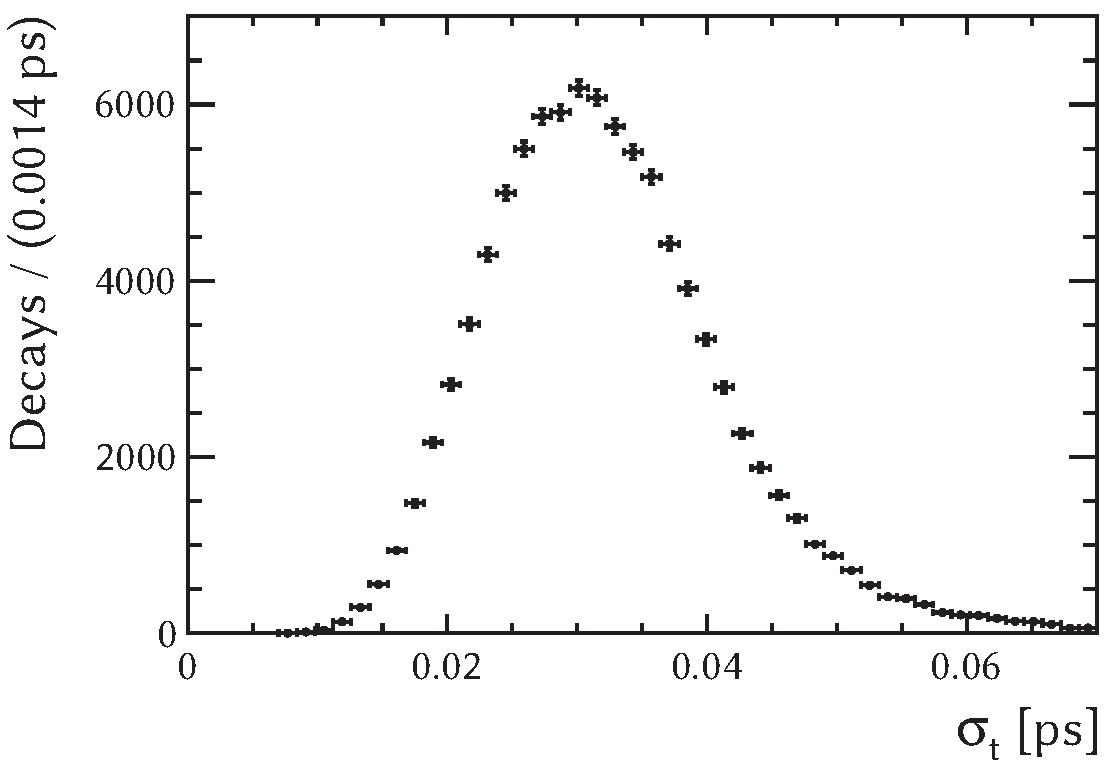
\includegraphics[width=0.5\textwidth]{graphics/analysis/sigmat}
  \caption{Distribution of \BstoJpsiKK{} signal decays in the estimated decay-time uncertainty.}
  \label{fig:sigmat}
\end{figure}

Decay-time resolution is included in the model for the signal decay by convolving the theoretical model with the model for the difference
between the measured time and the true time. This convolution is the integral of the two-dimensional PDF of the true and measured decay
times over all possible values of the former:
\begin{equation}
  P_\text{meas}(t_\text{meas}, \Omega)
    \equiv \int_0^\infty \ud t_\text{true}\, R(t_\text{meas} - t_\text{true}|\sigmat)\, P_\text{true}(t_\text{true}, \Omega)\ ,
\end{equation}
where $R$ is the PDF for the difference between the measured and true times, or the \emph{resolution model}. The resolution model is
conditional on $\sigmat$., i.e. normalized with respect to decay time for each individual value of $\sigmat$.

Although the resolution model is approximated by a Gaussian PDF with width $\sigmat$, a more sophisticated model is required to describe
the resolution in the PDF with sufficient precision. The model is a sum of two Gaussian PDFs with a common, non-zero mean and a width that
depends quadratically on $\sigmat$. The width of the first Gaussian PDF is approximately equal to $\sigmat$, while the width of the second
Gaussian PDF is roughly a factor two larger.

The double-Gaussian model is based on and validated with both simulated \BstoJpsiKK{} decays and prompt background decay candidates. Since
all tracks of prompt background candidates originate from the primary vertex, their ``true'' decay time is equal to zero and the
distribution of measured decay times is essentially the resolution model. Studies of the model and its parameters are described in detail
in references~\cite{Aaij:2015} and \cite{LHCb-ANA-2014-039}. The values of the resolution parameters are fixed in the fit of decay time and
angles. Uncertainties in the parameter values are propagated after the fit and accounted for as systematic uncertainties (see
Section~\ref{sec:result_syst}).


%%%%%%%%%%%%%%%%%%%%%%%%%%%
\subsection{Acceptance}
\label{subsec:ana_time_acc}
%%%%%%%%%%%%%%%%%%%%%%%%%%%

To account for the efficiencies of the decay-candidate reconstruction and selection processes, the expression for the differential decay
rate (Equation~\ref{eq:diffRateAngles}) is multiplied by an acceptance function before building a PDF.

\begin{figure}[htbp]
  \centering
  \begin{subfigure}{0.49\textwidth}
    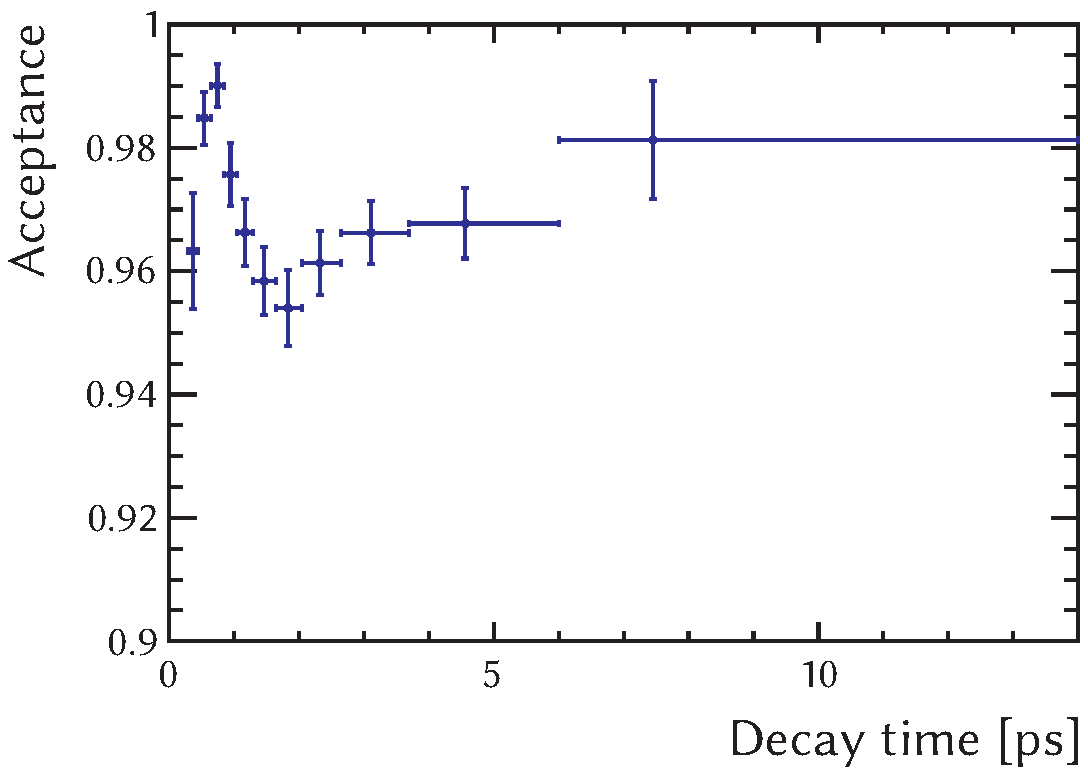
\includegraphics[width=\textwidth]{graphics/analysis/trigTimeAcc_2011_UB}
    \caption{}
    \label{fig:trigAcc_2011_UB}
  \end{subfigure}%
  \hfill%
  \begin{subfigure}{0.49\textwidth}
    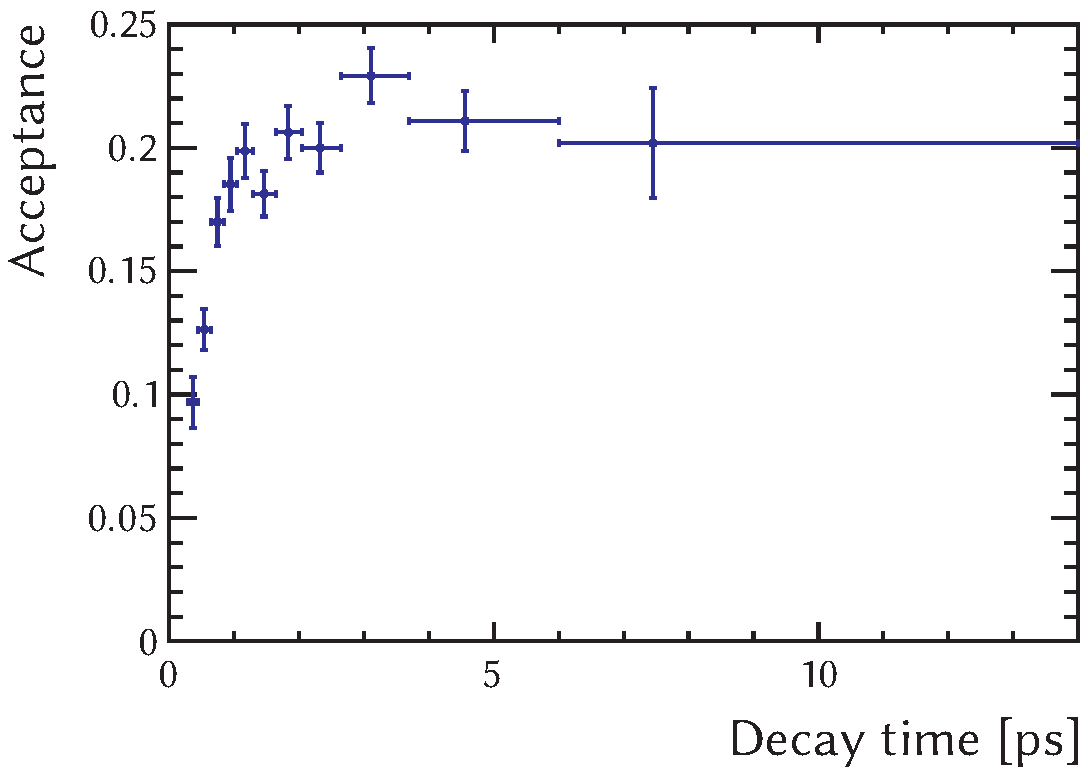
\includegraphics[width=\textwidth]{graphics/analysis/trigTimeAcc_2011_exclB}
    \caption{}
    \label{fig:trigAcc_2011_exclB}
  \end{subfigure}

  \vspace*{0.02\textwidth}
  \begin{subfigure}{0.49\textwidth}
    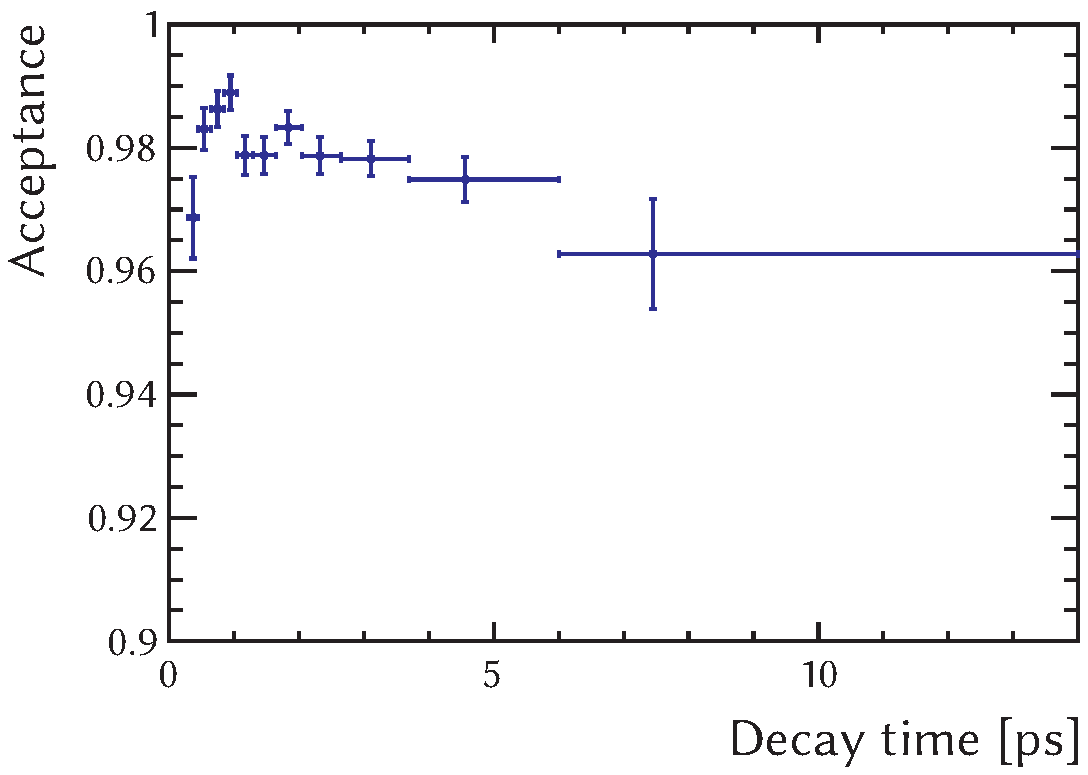
\includegraphics[width=\textwidth]{graphics/analysis/trigTimeAcc_2012_UB}
    \caption{}
    \label{fig:trigAcc_2012_UB}
  \end{subfigure}%
  \hfill%
  \begin{subfigure}{0.49\textwidth}
    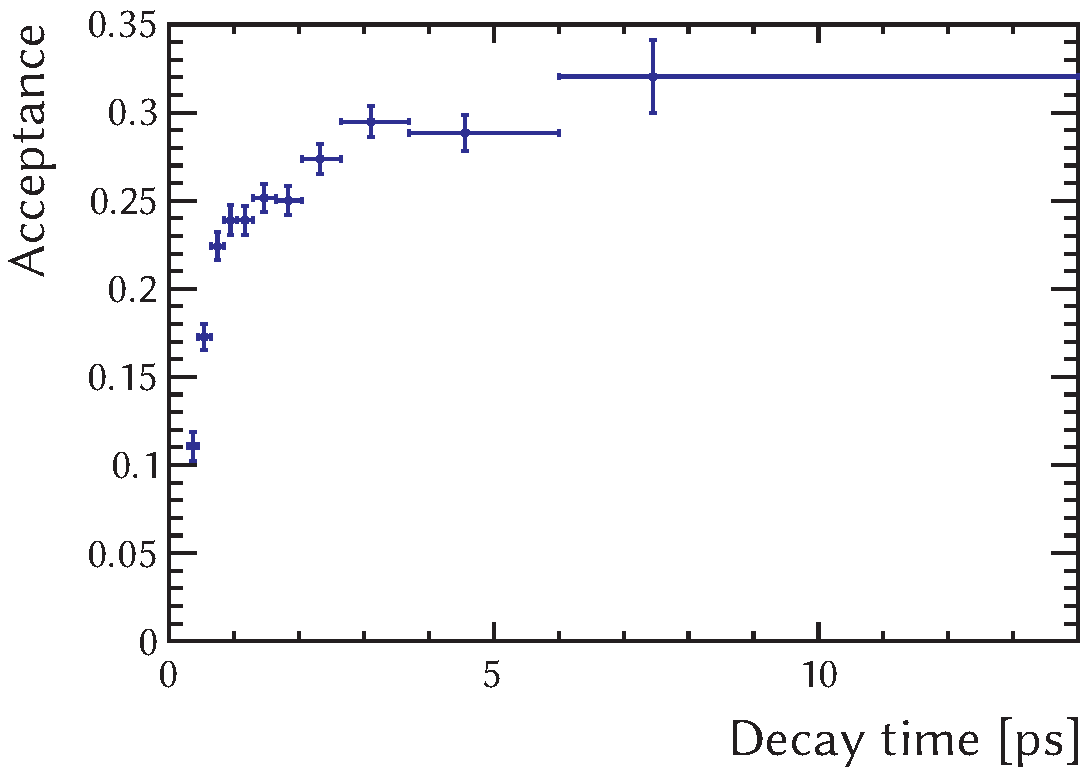
\includegraphics[width=\textwidth]{graphics/analysis/trigTimeAcc_2012_exclB}
    \caption{}
    \label{fig:trigAcc_2012_exclB}
  \end{subfigure}
  \caption{Trigger acceptance in bins of decay time for (a, b) the 2011 run and (c, d) the 2012 run
           and for (a, c) the HLT1-unbiased/HLT2-biased selection and (b, d) the exclusively HLT1-biased/HLT2-biased selection.
           Notice that the lower limit on the y-axis of the HLT1-unbiased/HLT2-biased graphs is 90\%.
           Because the absolute efficiency of the HLT1 selections is unknown, the scales of the efficiencies
           in the graphs are given with respect to the efficiency of the HLT1-unbiased selection.}
  \label{fig:trigAcc}
\end{figure}

